\begin{appendices}

%Some Table of Contents entry formatting
\addtocontents{toc}{\protect\renewcommand{\protect\cftchappresnum}{\appendixname\space}}
\addtocontents{toc}{\protect\renewcommand{\protect\cftchapnumwidth}{6em}}

%Begin individual appendices, separated as chapters

\chapter[\texorpdfstring{Linklet Kernel Language Specification}{Appendix A}]{Linklet Kernel Language Specification}
\label{appendix:linklet-kernel-language}

    \inputAppendixFigure{linklet-kernel-language-grammar.tex}

    \begin{figure}[h]
    \centering
    \fbox{
        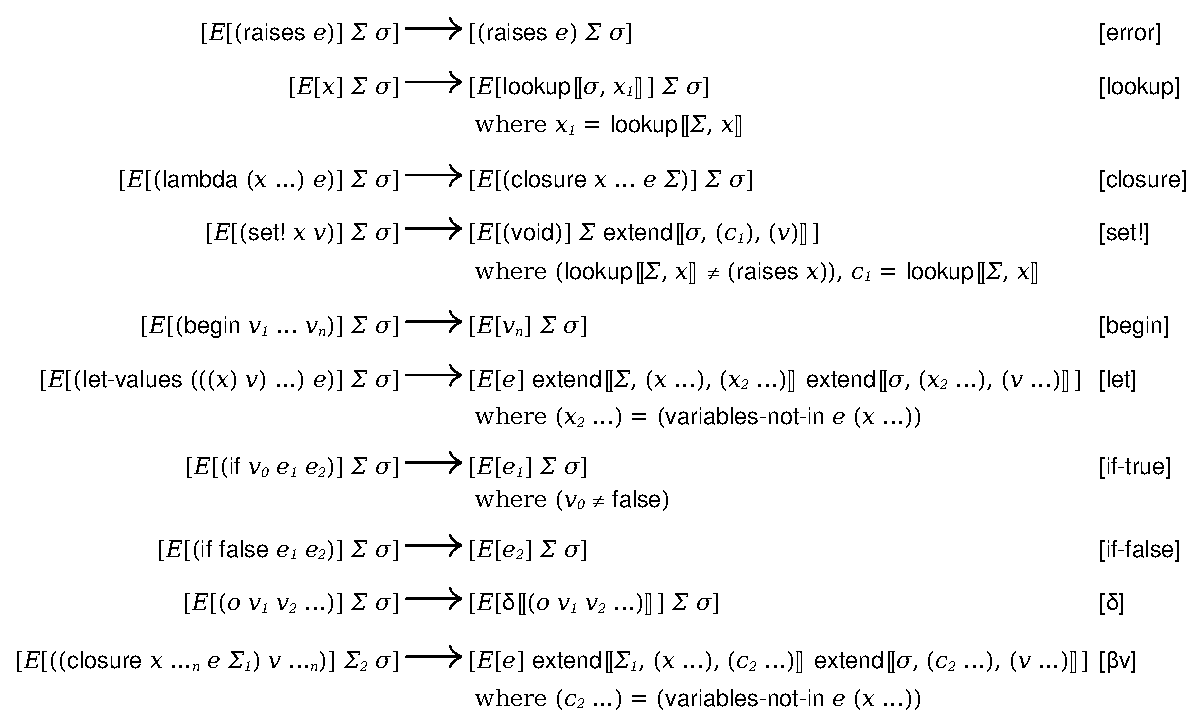
\includegraphics[scale=0.8]{sections/figures/rc-red-relation.eps}
    }
    \caption{Linklet Kernel Language standard reduction relation}
    \label{fig:rc-red-relation}
    \end{figure}

    \begin{figure}[h]
    \centering
    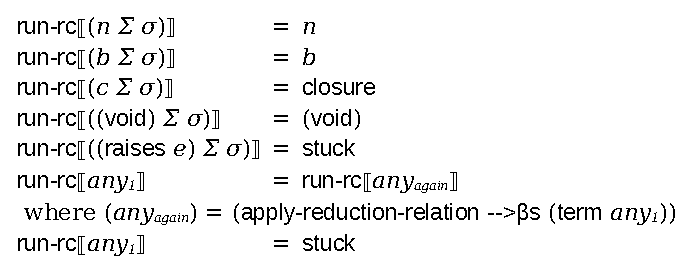
\includegraphics[scale=1]{sections/figures/rc-run-rc.eps}
    \caption{Linklet Kernel Language evaluator}
    \label{fig:rc-run-rc}
    \end{figure}


\chapter[\texorpdfstring{Complete Reduction Steps for Top-level Example Program}{Appendix B}]{Complete Reduction Steps for Top-level Example Program}
\label{appendix:formal-reduction-steps-toplevel-example}

    \inputAppendixFigure{complete-toplevel-example-step-by-step-formal.tex}

\chapter[\texorpdfstring{PLT Redex Model for Linklet Semantics}{Appendix C}]{PLT Redex Model for Linklet Semantics}
\label{appendix:linklet-semantics-model-redex-code}

    \begin{figure-here}
        Executable PLT Redex code for linklet model.
    \end{figure-here}

\chapter[\texorpdfstring{PLT Redex Model for CEK \& Stackful Hybrid Computation}
                          {Appendix D}]{PLT Redex Model for CEK \& Stackful Hybrid Computation}
\label{appendix:cek-stackful-redex}

    \begin{figure}[!h]
        \centering
        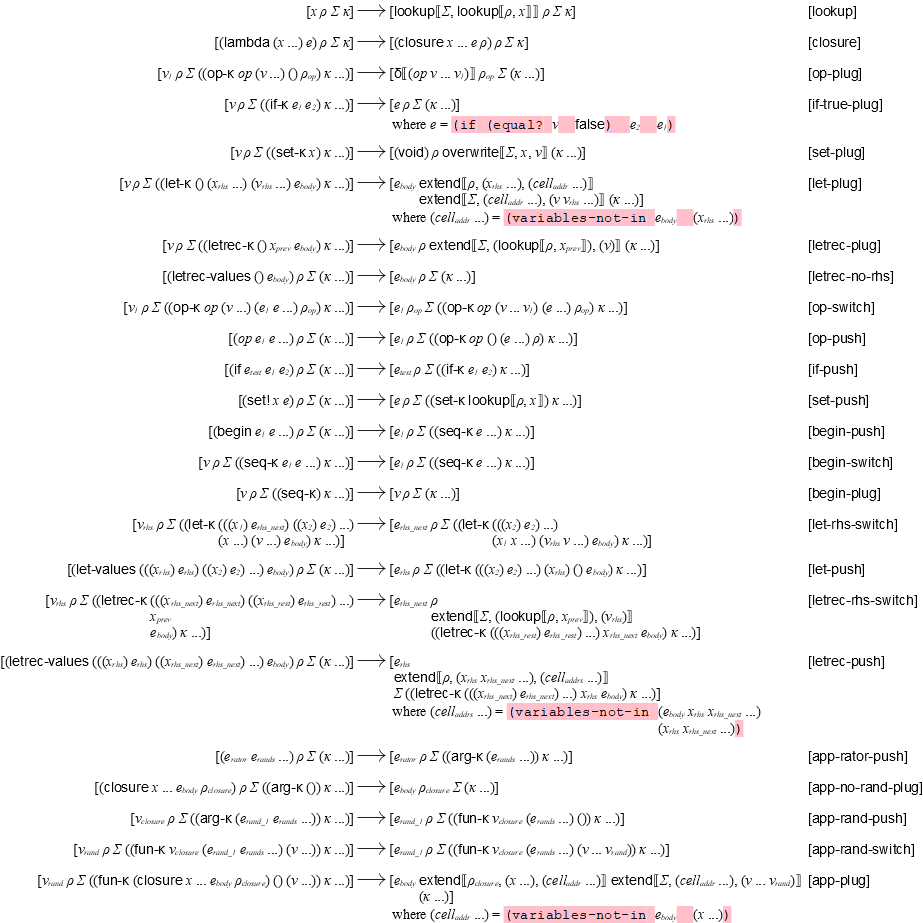
\includegraphics[scale=0.4]{sections/figures/cek-reduction-relation.png}
        \caption{CEK Reduction Relation [PLACEHOLDER]}
        \label{fig:cek-reduction-relation-redacted}
    \end{figure}

    \inputAppendixFigure{cek-reduction-relation-redacted}

    \begin{figure}[!h]
        \centering
        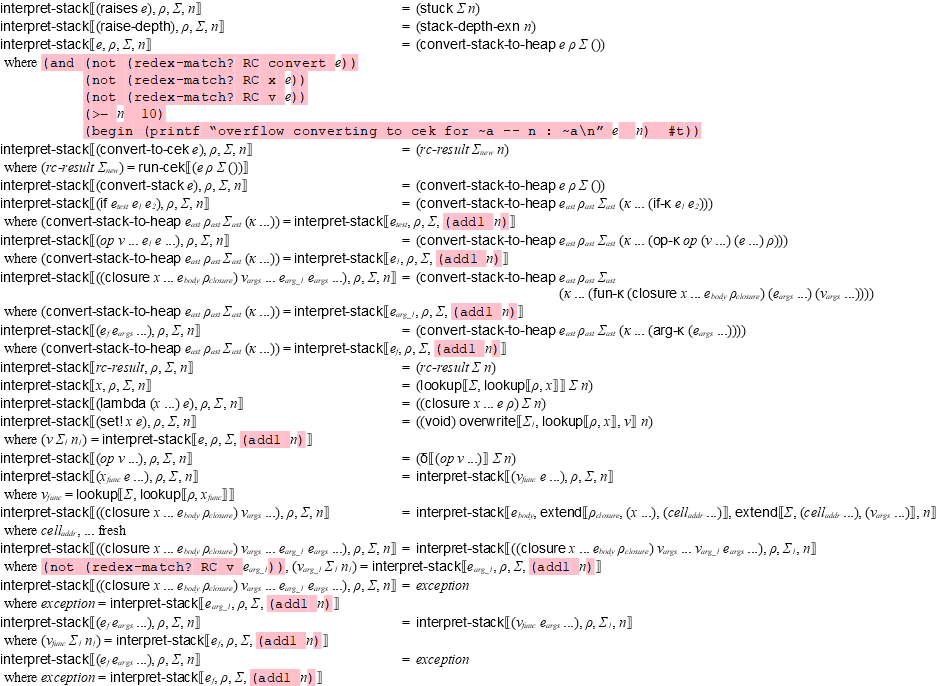
\includegraphics[scale=0.4]{sections/figures/interpret-stack-redacted.png}
        \caption{Stackful Model (Redacted) [PLACEHOLDER]}
        \label{fig:interpret-stack-redacted}
    \end{figure}

    \begin{figure}[!h]
        \centering
        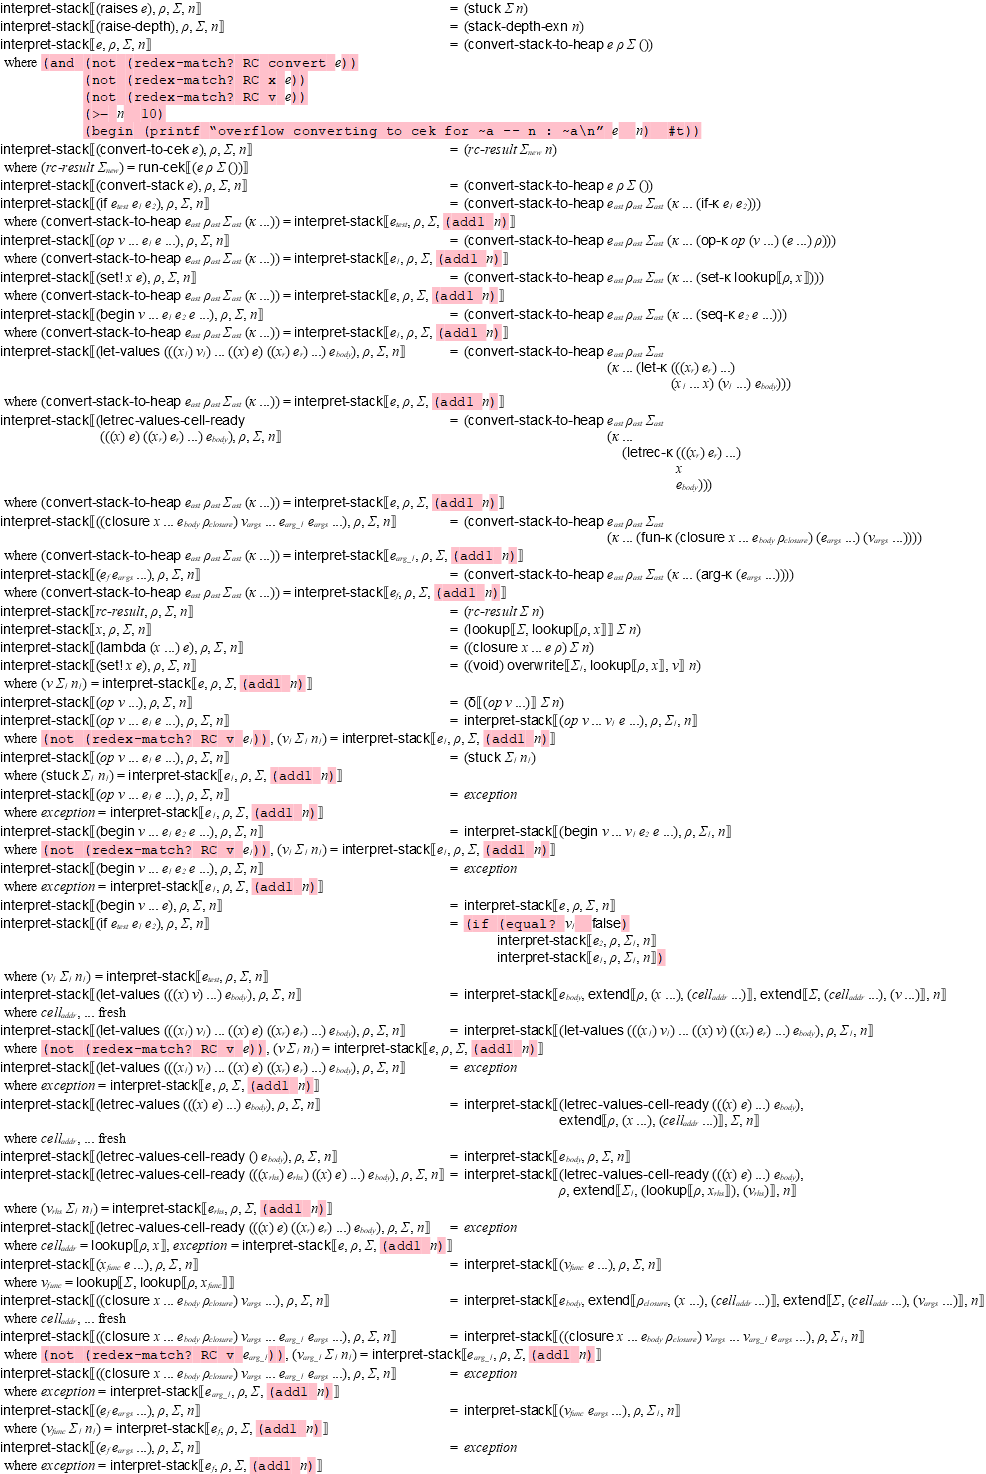
\includegraphics[scale=0.4]{sections/figures/interpret-stack-full.png}
        \caption{Stackful Model [PLACEHOLDER]}
        \label{fig:interpret-stack-full}
    \end{figure}

% \chapter{Data Processing}
% Lorem ipsum dolor sit amet, consectetur adipiscing elit, sed do eiusmod tempor incididunt ut labore et dolore magna aliqua. Ut enim ad minim veniam, quis nostrud exercitation ullamco laboris nisi ut aliquip ex ea commodo consequat. Duis aute irure dolor in reprehenderit in voluptate velit esse cillum dolore eu fugiat nulla pariatur. Excepteur sint occaecat cupidatat non proident, sunt in culpa qui officia deserunt mollit anim id est laborum.

\end{appendices}